\documentclass[table]{beamer}
%[]中可以使用handout、trancompress等参数

%指定beamer的模式与主题
\mode<presentation>
{
  \usetheme{Berkeley}
%\usetheme{Boadilla}
%\usecolortheme{default}
%\usecolortheme{orchid}
%\usecolortheme{whale}
%\usefonttheme{professionalfonts}
}

%\usetheme{Madrid}
%这里还可以选择别的主题:Bergen, Boadilla, Madrid, AnnArbor, CambridgeUS, Pittsburgh, Rochester, Warsaw, ...
%有导航栏的Antibes, JuanLesPins, Montpellier, ...
%有内容的Berkeley, PaloAlto, Goettingen, Marburg, Hannover, ...
%有最小导航栏的Berlin, Ilmenau, Dresden, Darmstadt, Frankfurt, Singapore, Szeged, ...
%有章和节表单的Copenhagen, Luebeck, Malmoe, Warsaw, ...

%\usecolortheme{default}
%设置内部颜色主题(这些主题一般改变block里的颜色);这个主题一般选择动物来命名
%这里还可以选择别的颜色主题,如默认的和有特别目的的颜色主题default,structure,sidebartab,全颜色主题albatross,beetle,crane,dove,fly,seagull,wolverine,beaver

%\usecolortheme{orchid}
%设置外部颜色主题(这些主题一般改变title里的颜色);这个主题一般选择植物来命名
%这里还可以选择别的颜色主题,如默认的和有特别目的的颜色主题lily,orchid,rose

%\usecolortheme{whale}
%设置字体主题;这个主题一般选择海洋动物来命名
%这里还可以选择别的颜色主题,如默认的和有特别目的的颜色主题whale,seahorse,dolphin

%\usefonttheme{professionalfonts}
%类似的还可以定义structurebold,structuresmallcapsserif,professionalfonts


% 控制 beamer 的风格,可以根据自己的爱好修改
%\usepackage{beamerthemesplit} %使用 split 风格
%\usepackage{beamerthemeshadow} %使用 shadow 风格
%\usepackage[width=2cm,dark,tab]{beamerthemesidebar}


% 设定英文字体
\usepackage{fontspec}
\setmainfont{WenQuanYi Micro Hei}
%~ \setmainfont{Times New Roman}
%~ \setsansfont{Arial}
%~ \setmonofont{Courier New}

% 设定中文字体
\usepackage[BoldFont,SlantFont,CJKchecksingle,CJKnumber]{xeCJK}
%~ \setCJKmainfont[BoldFont={Adobe Heiti Std},ItalicFont={Adobe Kaiti Std}]{Adobe Song Std}

\setCJKmainfont{WenQuanYi Micro Hei}%[BoldFont={WenQuanYi Micro Hei},ItalicFont={WenQuanYi Micro Hei}]
\setCJKsansfont{WenQuanYi Micro Hei}
\setCJKmonofont{WenQuanYi Micro Hei}

\punctstyle{hangmobanjiao}

\defaultfontfeatures{Mapping=tex-text}
\usepackage{xunicode}
\usepackage{xltxtra}

\XeTeXlinebreaklocale "zh"
\XeTeXlinebreakskip = 0pt plus 1pt minus 0.1pt

\usepackage{setspace}
\usepackage{booktabs}
\usepackage{colortbl,xcolor}
\usepackage{hyperref}
%\hypersetup{xetex,bookmarksnumbered=true,bookmarksopen=true,pdfborder=1,breaklinks,colorlinks,linkcolor=blue,filecolor=black,urlcolor=cyan,citecolor=green}
\hypersetup{xetex,bookmarksnumbered=true,bookmarksopen=true,pdfborder=1,breaklinks,colorlinks,linkcolor=cyan,filecolor=black,urlcolor=blue,citecolor=green}

% 插入图片
\usepackage{graphicx}
% 指定存储图片的路径(当前目录下的figures文件夹)
\graphicspath{{figures/}}

% 可能用到的包
\usepackage{amsmath,amssymb}
\usepackage{multimedia}
\usepackage{multicol}

% 定义一些自选的模板,包括背景、图标、导航条和页脚等,修改要慎重
% 设置背景渐变由10%的红变成10%的结构颜色
%\beamertemplateshadingbackground{red!10}{structure!10}
%\beamertemplatesolidbackgroundcolor{white!90!blue}
% 使所有隐藏的文本完全透明、动态,而且动态的范围很小
\beamertemplatetransparentcovereddynamic
% 使itemize环境中变成小球,这是一种视觉效果
\beamertemplateballitem
% 为所有已编号的部分设置一个章节目录,并且编号显示成小球
\beamertemplatenumberedballsectiontoc
% 将每一页的要素的要素名设成加粗字体
\beamertemplateboldpartpage

% item逐步显示时,使已经出现的item、正在显示的item、将要出现的item呈现不同颜色
\def\hilite<#1>{
 \temporal<#1>{\color{gray}}{\color{blue}}
    {\color{blue!25}}
}

% 自定义彩色块状结构的颜色
\setbeamercolor{bgcolor}{fg=yellow,bg=cyan}

% 在表格、图片等得标题中显示编号
\setbeamertemplate{caption}[numbered]

% 打开PDF后直接全屏
\hypersetup{pdfpagemode={FullScreen}}

% 使用 \part,\section,\subsection 等命令组织文档结构
% 使用 \frame 命令制作幻灯片
\usepackage{indentfirst}%段首缩进
%~ \usepackage{algorithm}
%~ \usepackage{algorithmic}
\begin{document}

\logo{
\includegraphics[height=0.12\textwidth]{sjtu.jpg}}
\title[题目简写]{论文题目全称}
\author[Author]{作者}
\institute[SJTU]{Shanghai Jiao Tong University\\ Department of XX\\ email}
\date{\today}

% 定义目录页
\AtBeginPart{
  \frame{
    \frametitle{\partpage}
    \begin{multicols}{2}% 如果目录过长,可以打开这个选项分两栏显示
      \tableofcontents % 使用这个命令自动生成目录
    \end{multicols}
  }  
}

% 在每个Section前都会加入的Frame
\AtBeginSection[]
{
  \begin{frame}<beamer>
    \frametitle{}
	\setcounter{tocdepth}{2}
    \tableofcontents[currentsection,currentsubsection]
  \end{frame}
}
% 在每个Subsection前都会加入的Frame
\AtBeginSubsection[]
{
  \begin{frame}<beamer>
%\begin{frame}<handout:0> % handout:0 表示只在手稿中出现
    \frametitle{}
	\setcounter{tocdepth}{2}
    \tableofcontents[currentsection,currentsubsection]
% 显示在目录中加亮的当前章节
  \end{frame}
}
\numberwithin{equation}{section}%使公式编号关联至章节
\setbeamertemplate{theorems}[numbered]%显示定理编号






%%%%%%%%%%%%%%%%%%%%%%%%%%%%%%%%%%%%%%%配置完成,以下为正文%%%%%%%%%%%%%%%%%%%%%%%%%%%%%%%%%%%%%%%
\begin{frame}
  \titlepage
\end{frame}

\begin{frame}{大纲}
  \setcounter{tocdepth}{2}
  \tableofcontents
\end{frame}





%%%%%%%%%%%%%%%%%%%%%%%%%%%%%%%%%%%%%%%第一章%%%%%%%%%%%%%%%%%%%%%%%%%%
\section{第一章}
\subsection{1.1}
\frame{
    \frametitle{带编号的公式示例}
    \begin{equation}
    \begin{split}
	a_{i}^{T}X \leq b_{i},\ i=1,2,...,n\\
	0 \leq x_{i} \leq P_{i},\ i=1,2,..  .,N
    \end{split}
    \end{equation}
}

\subsection{1.2}
\frame{
    \frametitle{各条依次显示示例}
    \begin{itemize}
	\item <1-> 第一条\\
	\item <2-> 第二条\\
    ......
    \end{itemize}
}

\frame{
    \frametitle{带编号列表示例}
    \begin{enumerate}
    \item aaa
    \item bbb\\
    ...
    \end{enumerate}
}



%%%%%%%%%%%%%%%%%%%%%%%%%%%%%第二章%%%%%%%%%%%%%%%%%%%%%%%%%%%%%%%%% 
\section{第二章}
\subsection{2.1}
\begin{frame}{插图示例}
    \centering{ 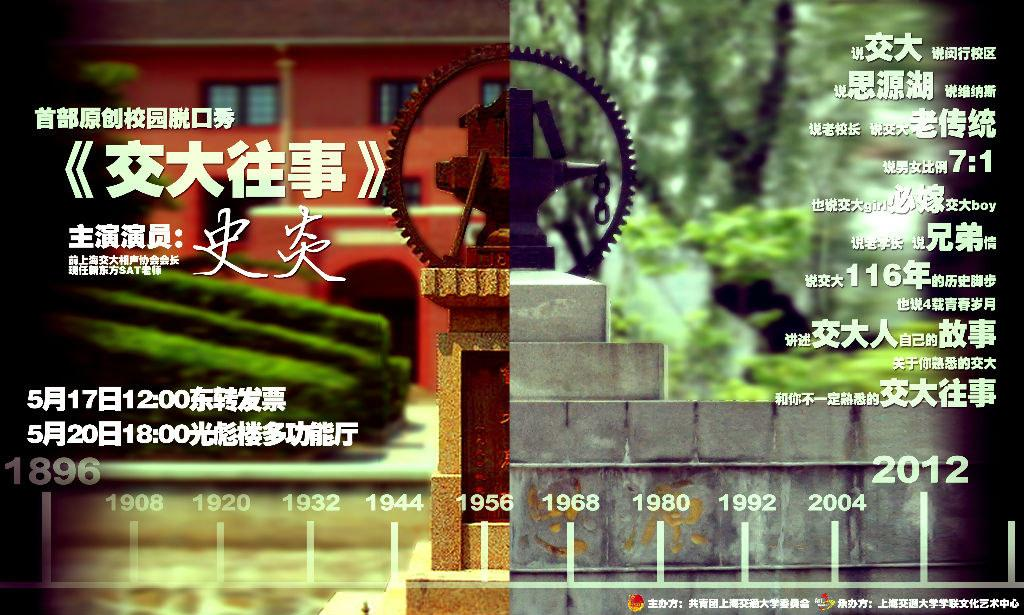
\includegraphics[width=10.5cm]{jdws.jpg} }%图片放于figures文件夹
\end{frame}

\subsection{2.2}
\frame{
    \frametitle{显示公式示例}
     \begin{theorem}[定理名称]\label{dl}%可以用\label{}和ref{}引用定理
    XXX定理
    \end{theorem}
}

\subsection{2.3}
\begin{frame}{表格示例}
% Table generated by Excel2LaTeX from sheet 'Sheet1' 推荐用excel2latex直接生成表格的tex代码
\begin{table}[htbp]
  \centering
  \caption{表格标题}
    \begin{tabular}{rrrrr}
    \addlinespace
    \toprule
          & c1    & c2    & c3    & c4 \\
    \midrule
    r1    & a     & e     & i     & m \\
    r2    & b     & f     & j     & n \\
    r3    & c     & g     & k     & o \\
    r4    & d     & h     & l     & p \\
    \bottomrule
    \end{tabular}%
  \label{tab:addlabel}%
\end{table}%
\end{frame}





\end{document}
